\documentclass[tikz, preview]{standalone}

\usepackage{amsfonts, amsthm, amssymb, amsmath, stmaryrd, etoolbox}
\usepackage{tikz}
\usetikzlibrary{matrix,arrows}

\begin{document}
\[
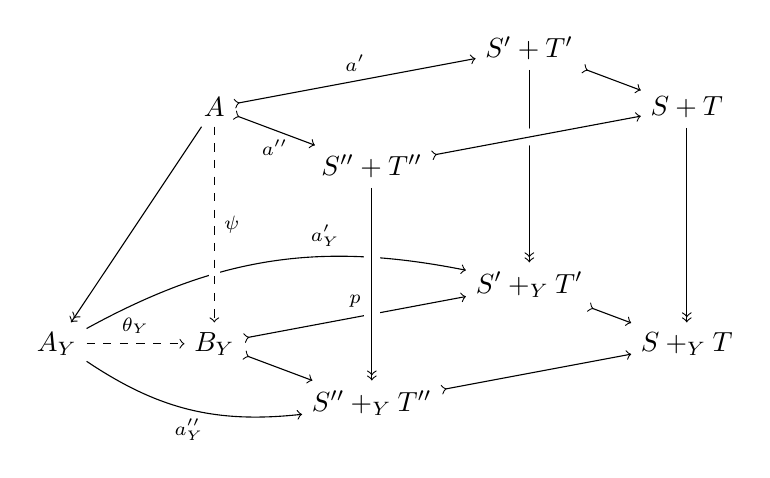
\begin{tikzpicture}
\node (A) at (2,3) {$A$};
\node (Ay) at (0,0) {$A_Y$};
\node (By) at (2,0) {$B_Y$};
\node (ST) at (8,3) {$S+T$};
\node (ST') at (6,3.75) {$S'+T'$};
\node (ST'') at (4,2.25) {$S''+T''$};
\node (SYT) at (8,0) {$S+_YT$};
\node (SYT') at (6,0.75) {$S'+_YT'$};
\node (SYT'') at (4,-0.75) {$S''+_YT''$};
%
\draw [->>] (A) edge (Ay);
\draw [font=\scriptsize,>->] (A) edge node[below] {$a''$} (ST'');
\draw [font=\scriptsize,>->] (A) edge node[above] {$a'$} (ST');
\draw [font=\scriptsize,->] (Ay) edge[bend left=20,pos=0.65] node[above] {$a'_Y$} (SYT');
\draw [font=\scriptsize,->] (Ay) edge[dashed] node[above] {$\theta_Y$} (By);
\draw [font=\scriptsize,->] (Ay) edge[bend right=20] node[below] {$a''_Y$} (SYT'');
\draw [font=\scriptsize,>->] (By) edge node[above] {$p$} (SYT');
\draw [>->] (By) edge (SYT'');
\draw [->>] (ST') edge (SYT');
\draw [>->] (ST') edge (ST);
\draw [>->] (ST'') edge (ST);
\draw [->>] (ST) edge (SYT);
\draw [>->] (SYT') edge (SYT);
\draw [>->] (SYT'') edge (SYT);
%
\draw [->] (A) edge[white,line width=4pt] (By);
\draw [font=\scriptsize,->] (A) edge[dashed] node[right] {$\psi$} (By);
\draw [->] (ST'') edge[white,line width=6pt] (ST);
\draw [>->] (ST'') edge (ST);
\draw [->] (ST'') edge[white,line width=6pt] (SYT'');
\draw [->>] (ST'') edge (SYT'');
\end{tikzpicture}
\]
\end{document}
